\chapter{Quantum Confinement and Superposition}

In quantum mechanics, particles can be `spatially confined' to a given energy potential where the energy levels of the confined particles will not remain continuous but instead are instead quantized.
Quantum mechanics allows us to obtain the wave functions of the confined particle and their discrete set of energy levels -- such kinds of effects appear when the dimensions of the potential approach the deBroglie wavelength of particle. These effects are the basis for several semiconductor devices.

In this lab, the infinite square well (often called ``particle in a box'') problem was investigated. This problem provides several illustrations of the properties of wave functions whilst being one of the less troublesome problems to solve.

\begin{figure}[h]
    \centering
    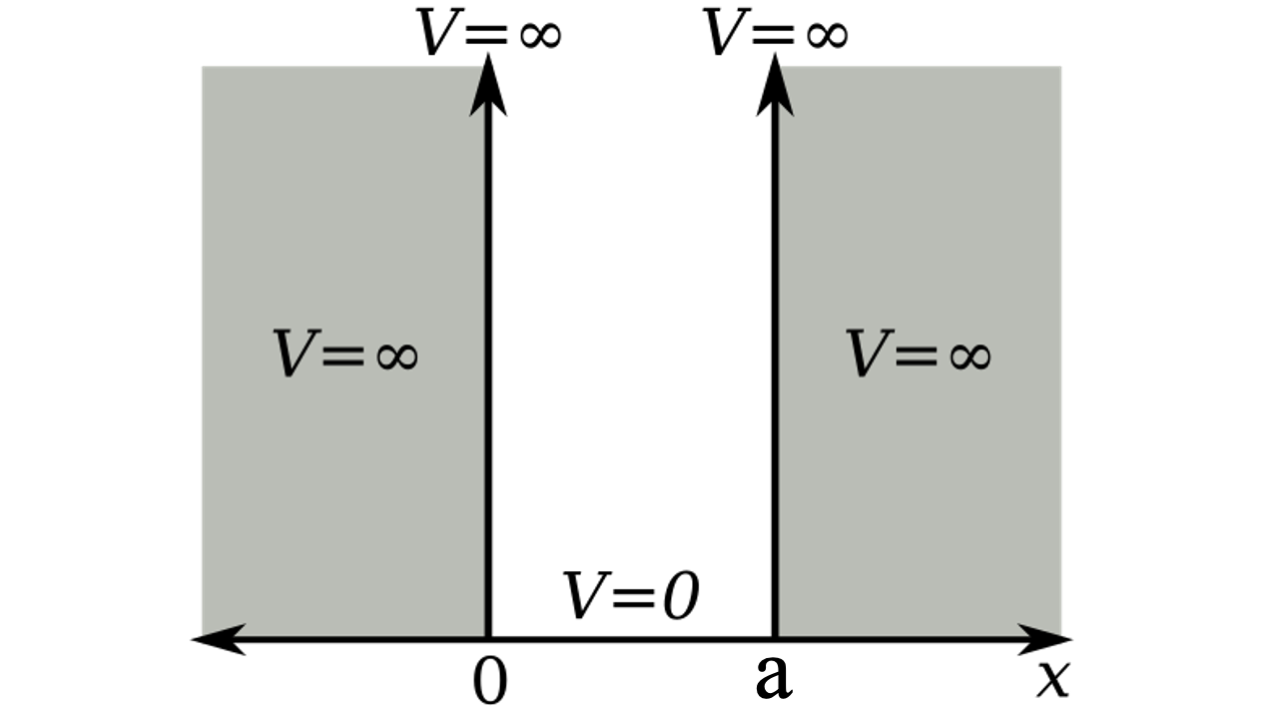
\includegraphics[width=0.5\textwidth]{lab1/images/pIAB.png}
    \captionsetup{font = it, labelfont = bf, width=.91\linewidth, justification=centering}
    \caption{Illustration of the ``particle in a box'' problem -- based on image from:\\ https://en.wikipedia.org/wiki/Particle\_in\_a\_box\#/media/File:Infinite\_potential\_well-en.svg}
    \label{fig:particleInABox}
\end{figure}

\[
  V(x) = \begin{cases}
  0 & 0 < x < a\\
  \infty & \text{elsewhere}
\end{cases}
\]
   
\section{Results}
\subsection{Energy Eigenvalues}
To determine the energy of the quantised states within the potential well, the time-independent one-dimensional Schrödinger equation must be considered:

$$E_n \psi_n (x) = \frac{-\hbar ^{2}}{2m}\frac{\delta^{2}}{\delta x^{2}}\psi_n (x) + V(x)\psi_n (x)$$
where $\hbar$ is the reduced Planck Constant, $m$ is the mass of the particle, $\psi_n (x)$ is the wavefunction, $V(x)$ is the potential, $E_n$ is the energy level and x is the position along the x-axis. 

$V(x)=0$ in the potential well: 

\begin{equation} \label{eq:shrod}
\therefore E_n \psi_n (x) = \frac{-\hbar ^{2}}{2m}\frac{\delta^{2}}{\delta x^{2}}\psi_n (x)
\end{equation}

Substituting $\psi_n (x)$ (the derivation for this eigenfunction can be found in Section~\ref{sec:eigenFunction}):
\begin{align*}
E_n \psi_n (x) &= \frac{-\hbar ^{2}}{2m}\frac{\delta^{2}}{\delta x^{2}}\Bigg(\sqrt{\frac{2}{a}}\sin\Big(\frac{n\pi x}{a}\Big)\Bigg)\\
E_n \psi_n (x) &= \frac{-\hbar ^{2}}{2m}\Big(\frac{n\pi}{a}\Big)^{2}\Bigg(\sqrt{\frac{2}{a}}\sin\Big(\frac{n\pi x}{a}\Big)\Bigg)\\
E_n \psi_n (x) &= \frac{\hbar ^{2}}{2m}\Big(\frac{n\pi}{a}\Big)^{2}\psi_n (x)\\
E_n &= \frac{\hbar ^{2}}{2m}\Big(\frac{n\pi}{a}\Big)^{2} & \text{where } n \in \mathbb{N}
\end{align*}

The energy eigenvalues for a well of width a=0.1nm is shown in Figure \ref{fig:eigenEnergy} for ($n=1$ to $n=5$)

\begin{figure}[h]
    \centering
    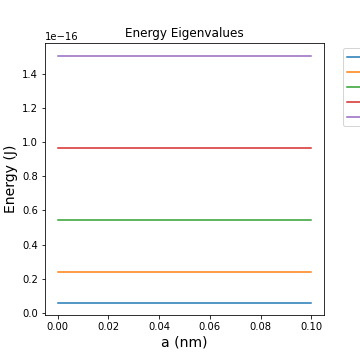
\includegraphics[width=0.4\textwidth]{lab1/images/eigenvaluesEnergy.png}
    \captionsetup{font = it, labelfont = bf, width=.91\linewidth, justification=centering}
    \caption{Plot showing the first 5 the discrete energy levels (n=1 to n=5) for a particle confined in a box of length 0.1nm} 
    \label{fig:eigenEnergy}
\end{figure}

The values for the quantised energies can be found in Table \ref{tab:qEnerergy}:

\begin{table}[h!]
\centering
\begin{tabular}{|l|l|l|}
\hline
\textbf{n} & \textbf{Energy (J)} \\ \hline
1 & 6.02467e-18 \\ \hline
2 & 2.40987e-17 \\ \hline
3 & 5.42220e-17 \\ \hline
4 & 9.63946e-17 \\ \hline
5 & 1.50617e-16 \\ \hline
\end{tabular}
\captionsetup{font = it, labelfont = bf, width=.91\linewidth, justification=centering}
\caption{Table showing the first 5 the discrete energy values (n=1 to n=5) for a particle confined in a box of length 0.1nm}
\label{tab:qEnerergy}
\end{table}

\subsection{Eigenfunctions}\label{sec:eigenFunction}
Equation \ref{eq:shrod} must firstly be rearranged to determine the eigenfunction -- aka the normalised wavefunction:

$$\frac{\delta^{2}}{\delta x^{2}}\psi (x) = \frac{-2m}{\hbar} E \psi (x) = -k^2 \psi (x)$$
$$\frac{\delta^{2}}{\delta x^{2}}\psi (x) + k^2 \psi (x) = 0$$
where $k=\sqrt{\frac{2mE}{\hbar}}$

To satisfy this second order homogeneous differential equation, the general equation is given by the following expression:

$$\psi (x) = A \sin(kx) + B \cos(kx)$$

Applying the boundary condition, $\psi (0)$=0:
\begin{align*}
\implies 0 &= A sin(0) + B cos(0)\\
 0 &= B\\
\therefore \psi (x) &= A sin(kx)
\end{align*}

Applying the boundary condition, $\psi (a)$=0:
\begin{align*}
\hspace{3.5cm} \implies 0 &= A sin(ka)\\
ka &= \pi n & \text{where } n \in \mathbb{N}\\
k &= \frac{\pi n}{a}\\
\therefore \psi_n (x) &= A sin(\frac{\pi n}{a}x)
\end{align*}

The eigenfunction must satisfy the following condition:

$$\int_{ -\infty}^{\infty}\psi_n (x)^{*}\psi_n (x)dx = 1$$
$$\int_{ -\infty}^{0}\psi_n (x)^{*}\psi_n (x)dx +\int_{0}^{a}\psi_n (x)^{*}\psi_n (x)dx + \int_{ a}^{\infty}\psi_n (x)^{*}\psi_n (x)dx= 1$$
\begin{align*}
\int_{ 0}^{a} A^{*} [sin(\frac{\pi n}{a}x)]^{*}A sin(\frac{\pi n}{a}x)dx = 1\\
A^{*}A\int_{ 0}^{a} [sin(\frac{\pi n}{a}x)]^{*}sin(\frac{\pi n}{a}x)dx = 1\\
\left | A \right |^2 \int_{ 0}^{a} sin(\frac{\pi n}{a}x) sin(\frac{\pi n}{a}x)dx = 1\\
\left | A \right |^2 \int_{ 0}^{a} sin^{2}(\frac{\pi n}{a}x)dx = 1\\
\left | A \right |^2 \left[\frac{x}{2}-\frac{asin(\frac{2 \pi nx}{a})}{4 \pi n}\right]_0^a= 1\\
\left | A \right |^2 [(\frac{a}{2}-0)-(0-0)]= 1\\
\left | A \right |^2 \frac{a}{2}= 1\\
\left | A \right | = \sqrt{\frac{2}{a}}
\end{align*}
$$\therefore \psi_n (x) = \sqrt{\frac{2}{a}} sin(\frac{\pi n}{a}x)$$

The normalised wavefunction, $\psi_n (x)$, for $n=1$ to $n=5$ is shown in Figure \ref{fig:normWave}.
\begin{figure}[h]
    \centering
    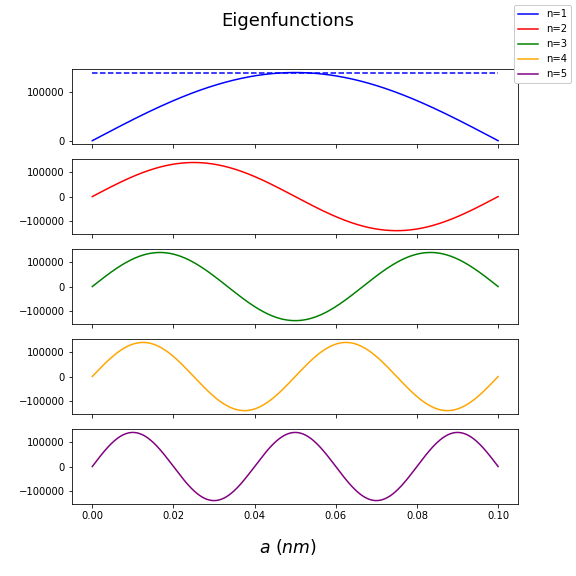
\includegraphics[width=0.5\textwidth]{lab1/images/normalisedWavefunction.png}
    \captionsetup{font = it, labelfont = bf, width=.91\linewidth, justification=centering}
    \caption{Plot showing the normalised wavefunctions for (n=1 to n=5) for a particle confined in a box of length 0.1nm}
    \label{fig:normWave}
\end{figure}

Figure \ref{fig:probDens} shows the probability density functions (PDFs), for $n=1$ to $n=5$:

$$P_n(x,dx) =\psi_n (x)^{*}\psi_n (x)dx =|\psi_n(x)|^{2}dx = \Bigg|\sqrt{\frac{2}{a}}\sin\Big(\frac{n\pi x}{a}\Big)\Bigg|^{2}dx  $$

\begin{figure}[H]
    \centering
    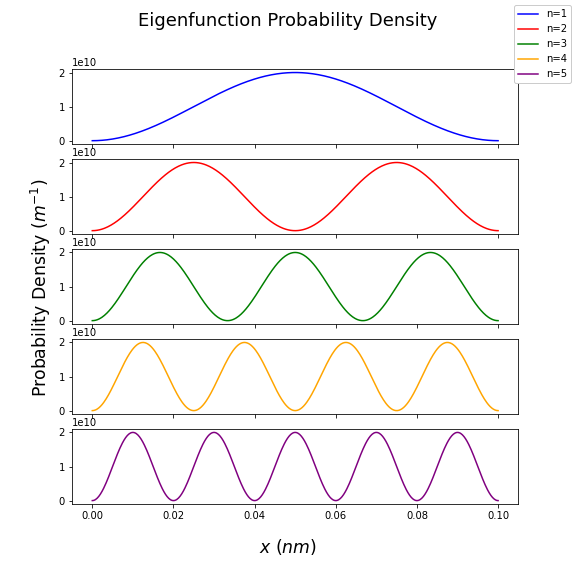
\includegraphics[width=0.5\textwidth]{lab1/images/probabilityDensity.png} %MISSING Y AXIS
    \captionsetup{font = it, labelfont = bf, width=.91\linewidth, justification=centering}
    \caption{Plot showing the probability density functions for (n=1 to n=5) for a particle confined in a box of length 0.1nm}
    \label{fig:probDens}
\end{figure}

\subsection{Superposition}

The eigenstates of the system plotted above are stationary. This means that when the system is in one of these eigenstates, all quantum mechanical observables are conserved in time (probability $P=|\Psi(x,t)|^2dx$ is independent of $\phi(t)$, meaning $P=|\psi(x)|^2dx$).

Superpositons of eigenfunctions are not stationary. To observe their non-stationary behaviours, namely, their time evolution we must calculate the superposition state for two states. The wavefunction for one state is given by:

$$\Psi_n (x,t) = \psi_n (x)\phi_n (t)$$
where $\psi_n (x)= \sqrt{\frac{2}{a}} sin(\frac{\pi n}{a}x)$ and $\phi_n (t)= e^{-i \omega t}$

The superposition state is therefore given by:
\begin{equation} \label{eq:superPos}
\Psi_s (x,t) = \psi_n (x)e^{-i \omega_{1} t} + \psi_m (x)e^{-i \omega_{2} t}
\end{equation}

This superposition wavefunction needs to be normalised, i. e.:
$$\int_{ -\infty}^{\infty} A^{*} \Psi_s (x,t)^{*} A\Psi_s (x,t)dx = 1$$
$$\left | A \right |^2 \int_{ -\infty}^{\infty} \Psi_s (x,t)^{*} \Psi_s (x,t)dx = 1$$

Given $\Psi_s (x,t)=0$ for $x<0, x>a$:
$$\left | A \right |^2 \int_{0}^{a} \Psi_s (x,t)^{*} \Psi_s (x,t)dx = 1$$

Substituting Equation \ref{eq:superPos}:
$$\left | A \right |^2 \int_{0}^{a} (\psi_n (x)^{*}e^{i \omega_{1} t} + \psi_m (x)^{*}e^{i \omega_{2} t}) (\psi_n (x)e^{-i \omega_{1} t} + \psi_m (x)e^{-i \omega_{2} t})dx = 1$$
$$\left | A \right |^2 \int_{0}^{a} (\left | \psi_n (x) \right |^2 + \left | \psi_m (x) \right |^2 + \psi_n (x)^{*}\psi_m (x)e^{-i(\omega_{2}- \omega_{1}) t} + \psi_m (x)^{*}\psi_n (x)e^{i(\omega_{2}- \omega_{1}) t})dx = 1$$

In this case $\psi_n (x)$ and $\psi_m (x)$ are completely real;\\
thus, $\psi_n (x)^{*} = \psi_n (x)$ and $\psi_m (x)^{*} = \psi_m (x)$:
$$ \left | A \right |^2 \int_{0}^{a}\left( \left | \psi_n (x) \right |^2 + \left | \psi_m (x) \right |^2 + \psi_m (x)\psi_n (x)(e^{-i(\omega_{2}- \omega_{1})t}+e^{i(\omega_{2}- \omega_{1})t})\right)dx = 1$$

Since $cos(x) = \frac{e^{ix}+e^{-ix}}{2}$:
$$ \left | A \right |^2 \int_{0}^{a}\left( \left | \psi_n (x) \right |^2 + \left | \psi_m (x) \right |^2 + \psi_m (x)\psi_n (x)(2\cos(\omega_{2}- \omega_{1})t)\right)dx = 1$$
$$ \left | A \right |^2 \int_{0}^{a}\left(\frac{2}{a} sin^{2}(\frac{\pi n}{a}x)+\frac{2}{a} sin^{2}(\frac{\pi m}{a}x)+\frac{4}{a} sin(\frac{\pi n}{a}x)sin(\frac{\pi m}{a}x)(\cos(\omega_{2}- \omega_{1})t)\right)dx = 1$$
$$...$$
$$\left | A \right |^2 \left( \frac{2}{a}\left(\frac{a}{2}\right) + \frac{2}{a}\left(\frac{a}{2}\right) + \frac{4}{a}\cos(\omega_{2}- \omega_{1})t\int_{0}^{a} sin(\frac{\pi n}{a}x)sin(\frac{\pi m}{a}x)dx \right)=1$$

$$\left | A \right |^2 \left( 1 + 1 + \frac{4}{a}\cos(\omega_{2}- \omega_{1})t(0) \right)=1$$
$$\left | A \right |^2 = \frac{1}{2}$$
$$\left | A \right | = \sqrt{\frac{1}{2}}$$
$$\therefore \Psi_s (x, t) = \sqrt{\frac{1}{2}} \left( \psi_n (x)e^{-i \omega_{1} t} + \psi_m (x)e^{-i \omega_{2} t}\right)$$

The real part of this superpositioned wavefunction was plotted as shown in Figure \ref{fig:superPosWave}.

\begin{figure}[h]
    \centering
    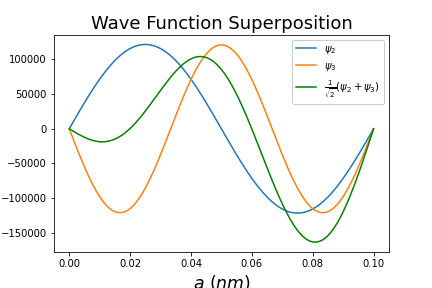
\includegraphics[width=0.65\textwidth]{lab1/images/superpositionWave.png}
    \captionsetup{font = it, labelfont = bf, width=.91\linewidth, justification=centering}
    \caption{Plot showing the two eigenstates, $\psi_2 (x)$ and $\psi_3 (x)$, and the superposition of both eigenstates for a particle confined in a box of length 0.1nm at time \textbf{t=1}}
    \label{fig:superPosWave}
\end{figure}

The probability distribution of the new wavefunction $\Psi_s(x,t)$ was then calculated and plotted at several different times to see how it evolves in time, shown in Figure \ref{fig:superPosPDF}.

$$P_s(x, t) = A^{*} \Psi_s (x, t)^{*} A\Psi_s (x, t)$$
$$P_s(x) = \left | A \right |^2 \Psi_s (x,t)^{*} \Psi_s (x,t)$$
$$P_s(x) = 0.5 (\psi_n (x)^{*}e^{i \omega_{1} t} + \psi_m (x)^{*}e^{i \omega_{2} t}) (\psi_n (x)e^{-i \omega_{1} t} + \psi_m (x)e^{-i \omega_{2} t})$$
$$P_s(x) = 0.5 (\left | \psi_n (x) \right |^2 + \left | \psi_m (x) \right |^2 + \psi_n (x)^{*}\psi_m (x)e^{-i(\omega_{2}- \omega_{1}) t} + \psi_m (x)^{*}\psi_n (x)e^{i(\omega_{2}- \omega_{1}) t})$$

As stated earlier $\psi_n (x)=\psi_n (x^{*})$ and $\psi_m (x)=\psi_m (x^{*})$:
$$\therefore P_s(x) =  0.5 (\left | \psi_n (x) \right |^2 + \left | \psi_m (x) \right |^2 + \psi_n (x)\psi_m (x)e^{-i(\omega_{2}- \omega_{1}) t} + \psi_m (x)\psi_n (x)e^{i(\omega_{2}- \omega_{1}) t})$$
$$P_s(x) = 0.5 (\left | \psi_n (x) \right |^2 + \left | \psi_m (x) \right |^2 + \psi_n (x)\psi_m (x)(e^{-i(\omega_{2}- \omega_{1}) t} + e^{i(\omega_{2}- \omega_{1}) t}))$$

Since $\cos(x)=\frac{e^{-ix}+e^{ix}}{2}$:
$$P_s(x) = 0.5 (\left | \psi_n (x) \right |^2 + \left | \psi_m (x) \right |^2 + \psi_n (x)\psi_m (x)(2\cos\omega t))$$
$$P_s(x) = 0.5 \left | \psi_n (x) \right |^2 + 0.5\left | \psi_m (x) \right |^2 + \psi_n (x)\psi_m (x)\cos\omega t$$

\begin{figure}[h]
    \centering
    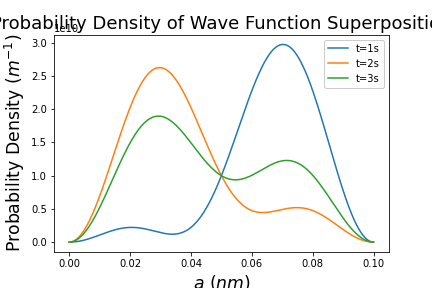
\includegraphics[width=0.75\textwidth]{lab1/images/superpositionPDF.png}
    \captionsetup{font = it, labelfont = bf, width=.91\linewidth, justification=centering}
    \caption{Probability density function for the superimposed state, $\Psi_s (x,t)$, plotted at various times}
    \label{fig:superPosPDF}
\end{figure}

\section{Comparison of Results with Theory}

The results from this lab is entirely based on theory so there are no discrepancies of the results with theory.

When calculating $E_n$ for $n=1,2,3,4,5$ it was clear to see that the ratio of $\frac{E_n}{E_1}$ is always equal to $n^{2}$. This can be proved mathematically by substituting $n=1$:
$$E_1 = \frac{\hbar ^{2}\pi^{2}}{2ma^{2}}$$

\begin{equation}\label{eq:energySpacing}
\implies E_n =  n^{2}E_1
\end{equation}
Equation \ref{eq:energySpacing} suggests that the energy levels must become more sparse as $n$ increases. This was seen in Figure~\ref{fig:eigenEnergy}.

All of the wave functions were 0 at the walls of the box, which means that the boundary conditions were always satisfied.

The peak of the wavefunctions had a value of $\approx \sqrt{2/L}$; this was the required amplitude to achieve a normalised wavefunction. The peak probability was subsequently found to be no higher than $2/L$, therefore the correct wavefunctions were achieved.

To ensure the correct PDF was achieved, the trapz function was used. This function calculated the area under the curve and was always found to be $\approx 1$. Thus confirming the amplitude of the wavefunction was calculated correctly. 

\section{Discussion}
\textbf{Question 1:}
\textit{After creating the energy-level diagram for up to $n=5$, create a code that finds the wavelengths of the photons emitted for all transitions beginning at state $n=3$ or less and ending at a lower energy state.}

The wavelength was found using the following equation:

\[\lambda = \frac{hc}{\Delta E}\]
where $\lambda$ is the wavelength of the photon, $h$ is Planks constant, $c$ is the speed of light and $\Delta E$ is the difference in energy eigenvalues.

The code and the output is shown below:

\begin{listing}[H]
\begin{minted}[
frame=lines,
framesep=2mm,
baselinestretch=1.2,
bgcolor=LightGray,
fontsize=\footnotesize,
linenos
]{python}

def wavelength(E):
    l = const.Planck*const.c/E
    return l

#Transition n=3 to n=2
print("n=3 to n=2 photon wavelength: ", 
      wavelength(Eigen_energies[2]-Eigen_energies[1]),"m")
#Transition n=3 to n=1
print("n=3 to n=1 photon wavelength: ", 
      wavelength(Eigen_energies[2]-Eigen_energies[0]),"m")
#Transition n=2 to n=1
print("n=2 to n=1 photon wavelength: ", 
      wavelength(Eigen_energies[1]-Eigen_energies[0]),"m")
\end{minted}
\end{listing}

\begin{lstlisting}[frame=single,style=base,backgroundcolor=\color{black}, basicstyle=\small]
@>>> n=3 to n=2 photon wavelength:  6.594375173013399e-09 m
>>> n=3 to n=1 photon wavelength:  4.1214844831333745e-09 m
>>> n=2 to n=1 photon wavelength:  1.0990625288355668e-08 m@
\end{lstlisting}


\section{Conclusions}
In this lab the particle in a well problem was analysed. The energy levels of a confined particle was investigated visualised using jupyter notebook. The interaction of wavefunctions at these energy levels was observed to obtain a deeper understanding of the nature of quantum particles. The objectives were met comfortably, therefore, no changes are required to meet them. 